\section{Struktur}
Softwarens struktur er bygget op omkring to sensorer som måler temperatursvingninger mellem rummet og vandrøret. I dette afsnit vil de enkelte funktionerne i softwaren blive beskrevet. 
\begin{figure}[h!]
  \centering
  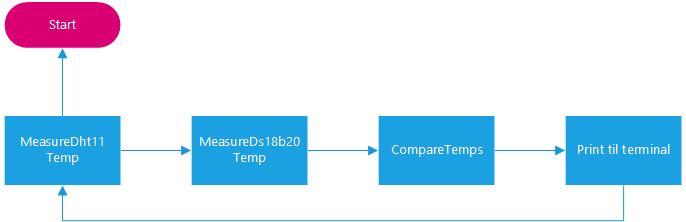
\includegraphics[width=0.5\textwidth]{figures/Fase1software2.png}
  \caption{Software flowchart.}
  \label{fase1flow}
\end{figure}
\fxnote{rediger flowchart så så pilen i start funktionen fra start og ikke imod start.}

\fxnote{kode i midten eller helt til venstre?(fjern centering)}

\begin{figure}[h!]
  \centering
  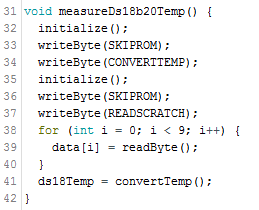
\includegraphics[width=0.5\textwidth]{figures/kode_measure_ds18b20.png}
  \caption{Funktion til aflæsning af temperatur fra DS18B20}
  \label{ds18b20Measure}
\end{figure}
Funktionen measureDs18b20Temp() er en samling af de nødvendige funktioner sensoren skal bruge for at sende en temperatur til mikroprocessoren, samt en funktion til at konvertere dataen, som modtages i hex, til et tal der kan vises.\newline
Temperaturen gemmes herefter i en integer, ds18Temp, som bruges senere, i compareTemps().\\\\

\begin{figure}[h!]
  \centering
  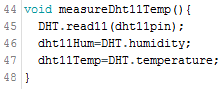
\includegraphics[width=0.5\textwidth]{figures/kode_measure_dht11.png}
  \caption{Funktion til aflæsning af temperatur fra DHT11}
  \label{dht11Measure}
\end{figure}
Denne funktion gemmer temperaturen og fugtigheden målt fra sensoren DHT11. Dette gøres gennem et bibliotek stillet til rådighed af Adafruit.\newline
\fxnote{nævn at denne også bruger 1-Wire og det ikke var nødvendigt at lave koden forfra her også?}
Disse gemmes i en integer hver, dog bliver fugtigheden ikke brugt.

\begin{figure}[h!]
  \centering
  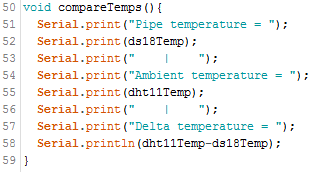
\includegraphics[width=0.5\textwidth]{figures/kode_compare.png}
  \caption{Funktion til sammenligning og print af temperatur}
  \label{compareTemp}
\end{figure}
For at få et overblik over dataen bliver begge temperaturer sendt til serielporten i funktionen compareTemps(). På samme linie bliver disse sammenlignet, så det er muligt at se forskellen på en ordentlig måde.



